\documentclass[11pt,a4paper]{article}
\usepackage[top=3cm, bottom=2cm, left=2cm, right=2cm]{geometry}
\usepackage[utf8]{inputenc}
\usepackage{amsmath, amsfonts, amssymb}
\usepackage{siunitx}
\usepackage[brazil]{babel}
\usepackage{graphicx}
\usepackage[margin=10pt,font={small, it},labelfont=bf, textfont=it]{caption}
\usepackage[dvipsnames, svgnames]{xcolor}
\DeclareCaptionFont{MediumOrchid}{\color[svgnames]{MediumOrchid}}
\usepackage[pdftex]{hyperref}
\usepackage{natbib}
\bibliographystyle{plainnat}
\bibpunct{\textcolor{MediumOrchid}{\textbf{[}}}{\textcolor{MediumOrchid}{\textbf{]}}}{,}{s}{}{}
\usepackage{color}
\usepackage{footnote}
\usepackage{setspace}
\usepackage{booktabs}
\usepackage{multirow}
\usepackage{subfigure}
\usepackage{fancyhdr}
\usepackage{leading}
\usepackage{indentfirst}
\usepackage{wrapfig}
\usepackage{mdframed}
\usepackage{etoolbox}
\usepackage[version=4]{mhchem}
\usepackage{enumitem}
\usepackage{caption}
\usepackage{titlesec}
\usepackage{tcolorbox}
\usepackage{tikz}
\usepackage{LobsterTwo}
\usepackage[T1]{fontenc}
\usepackage{fontspec}
\usepackage{txfonts}
\usepackage[bottom]{footmisc}

\makeatletter
\def\footnoterule{\kern-3pt\color{MediumOrchid}\hrule\@width0.6\textwidth height 0.8pt\kern2.6pt}
\makeatother

\renewcommand{\footnotelayout}{\itshape\color{black}}

\AtBeginEnvironment{equation}{\fontsize{13}{16}\selectfont}


\titleformat{\section}{\LobsterTwo\LARGE\color{CarnationPink}}{\thesection.}{1em}{}
\titleformat{\subsection}{\LobsterTwo\LARGE\color{CarnationPink}}{\thesubsection}{1em}{}


\DeclareCaptionLabelFormat{figuras}{\textcolor{DarkTurquoise}{Figura \arabic{figure}}}
\captionsetup[figure]{labelformat=figuras}

\makeatletter
\renewcommand\tagform@[1]{\maketag@@@{\color{CarnationPink}(#1)}}
\makeatother

\renewcommand{\theequation}{Eq. \arabic{equation}}
\renewcommand{\thefigure}{Fig. \arabic{figure}}
\renewcommand{\thesection}{\textcolor{CarnationPink}{\arabic{section}}}

\setlist[itemize]{label=\textcolor{CarnationPink}{$\mathbf{\square}$}}

\setlist[enumerate]{label=\textcolor{CarnationPink}{\arabic*.}, align=left}


\newcounter{exemplo}

\NewDocumentEnvironment{exemplo}{ O{} }{%
\allowbreak
\setlength{\parindent}{0pt}
  \begin{mdframed}[
  leftline=true,
  topline=false,
  rightline=false,
  bottomline=false,
  linewidth=2pt,
  linecolor=CarnationPink,
  frametitlerule=false,
  frametitlefont=\LobsterTwo\large\color{CarnationPink},
  frametitle={\color{CarnationPink}\LobsterTwo\large #1},
  ]
}{%
  \end{mdframed}
}

\setlength{\fboxsep}{5pt}
\setlength{\fboxrule}{1.5pt}
\usepackage{float}
\renewcommand{\thefootnote}{\alph{footnote}}
\usepackage{url}
\hypersetup{
	colorlinks=true,
	linkcolor=DarkTurquoise,
	filecolor=DarkTurquoise,      
	urlcolor=DarkTurquoise,
	citecolor=DarkTurquoise,
	pdftitle={Especialista em Física da Radioterapia}
}
\pagestyle{fancy}
\fancyhf{}
\renewcommand{\headrulewidth}{0pt}
\rfoot{Página \thepage}

\title{\LobsterTwo\Huge{Radioterapia}}
\author{\LobsterTwo\Large{Planejamento e Métricas Para Determinar a Qualidade do Plano}\nocite{*}}
\date{\LobsterTwo\textit{Dalila Mendonça}}
\begin{document}
	\maketitle

\section{Introdução}

	O objetivo geral do processo de planejamento do tratamento é fornecer a distribuição de dose ideal para o paciente, levando em consideração os seguintes fatores:

	\begin{enumerate}[label=\textcolor{CarnationPink}{(\roman*)}]
		\item Intenção do tratamento (curativo ou paliativo);
		\item Estágio da doença (extensão do envolvimento);
		\item Outras terapias (quimioterapia, hormônios, etc.);
		\item Tratamentos anteriores;
		\item Reprodutibilidade (imobilização, conforto do paciente);
		\item Entregabilidade (colisões, modulação); e
		\item Segurança (sensibilidade a mudanças, robustez).
	\end{enumerate}

	\begin{wrapfigure}{r}{0.4\textwidth}
		\centering
		\fcolorbox{DarkTurquoise}{white}{%
			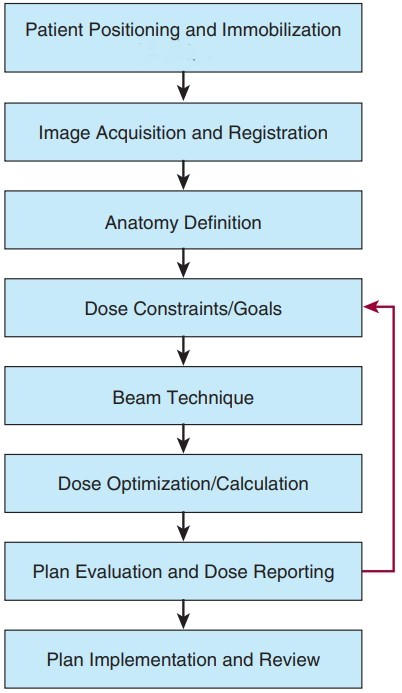
\includegraphics[width=0.3\textwidth]{Imagens/FluxogramadePlanejamento.jpg}
		}%
		\caption{Algoritmo do processo de planejamento.}
		\label{fig:FluxogramadePlanejamento}
	\end{wrapfigure}

	Desde o início, o médico, os técnicos de radioterapia, o físico médico e o dosimetrista devem ter uma comunicação clara sobre os fatores mencionados acima. O máximo de informações possível deve ser documentado no prontuário do paciente para que a sequência de eventos e o status atual do processo de tratamento sejam claros para todos. 
	
	Um esquema do processo de simulação e planejamento do tratamento é mostrado na \ref{fig:FluxogramadePlanejamento}. O fluxo começa com a imobilização e o setup garantindo reprodutibilidade e conforto do paciente. A comunicação é muito importante, como já dito anteriormente. Por exemplo, se um paciente foi submetido a uma cirurgia no ombro e não consegue elevar confortavelmente o braço acima da cabeça, outras estratégias de imobilização podem ser necessárias. Da mesma forma, se um paciente ficar agitado durante a simulação de TC devido à claustrofobia, o técnico precisará se comunicar com o médico e com a enfermagem para que sejam tomadas medidas para reduzir a ansiedade do paciente.

	A capacidade de reproduzir o tratamento de forma confiável ao longo de todo o curso é a chave para a administração bem-sucedida da radioterapia. O primeiro passo para alcançar esse objetivo é um setup e uma imobilização cuidadosa do paciente de modo que maximize o conforto enquanto restringe o movimento.

	Após o posicionamento do paciente, podem ser obtidas imagens que são usadas para definir os alvos e as estruturas críticas necessárias para planejar com segurança o curso do tratamento. Em muitos casos, estudos de imagem adicionais são usados para obter informações sobre a definição de tecidos moles, informações funcionais ou informações metabólicas que não estão disponíveis no conjunto de imagens primário. Esses conjuntos de imagens devem ser co-registrados para preservar a representação geométrica precisa dos dados.

	O contorno preciso do(s) alvo(s) e dos órgãos de risco (OAR) é fundamental para o desenvolvimento de um plano de tratamento de alta qualidade. Se os alvos forem contornados com muita liberdade, os OARs podem receber doses altas desnecessariamente. Da mesma forma, se os OARs forem expandidos em um grau inconsistente com a técnica de setup e localização usada, a dose no alvo pode ser desnecessariamente comprometida.

	

	A intenção médica de tratamento deve conter a dose total planejada e o fracionamento e deve informar as prioridades em relação aos objetivos e restrições de dose. O estágio da doença determinará a extensão da cobertura, como quais cadeias nodais precisam ser cobertas. Mais uma vez, a comunicação é importante. Por exemplo, se o médico disser ao dosimetrista que é aceitável comprometer a cobertura do alvo para garantir que todas os constraints para os OAR sejam atendidos, uma anotação deve ser feita no prontuário para que caso outro dosimetrista assumir o planejamento ou para o físico que revisar o plano também entenda os objetivos utilizados.

	Um plano deve ser consistente com as capacidades do sistema de entrega para que o tratamento seja entregue com segurança. Por exemplo, se for determinado que a reprodutibilidade do setup do paciente e da posição do isocentro é de 3 mm para uma determinada forma de imobilização e para técnica de imagem utilizada, as margens do plano devem refletir essas incertezas (ou seja, não utilizar margens de 1 mm).

	Depois que o contorno estiver finalizado e o método de entrega tiver sido definido, por exemplo, 3D ou radioterapia de intensidade modulada (IMRT), o plano pode ser otimizado. A otimização pode ser um processo manual de tentativa e erro nos casos de entrega conformacional 3D ou um processo de planejamento inverso para as entregas de IMRT. Em ambos os casos, os objetivos de dose desejados devem ser claramente definidos. O responsável pelo planejamento deve estar ciente das limitações do equipamento para evitar a criação de um plano que não pode ser entregue pelo linac. Algumas dessas limitações, como a velocidade do gantry, a taxa de dose, o número mínimo e máximo de unidades monitoras (MU), etc\dots,  podem ser inseridas no sistema de planejamento de tratamento (TPS) para evitar a criação de planos que excedam os limites operacionais do equipamento. Planos com alto grau de modulação podem levar os parâmetros do equipamento ao seu limite e, embora possam ser entregues, podem levar a um excesso de interlocks durante o tratamento.

	Após a otimização do plano, os vários constraints de dose e objetivos de cobertura do alvo são avaliadas para determinar se o plano é aceitável. Caso o plano não seja aceitável, os parâmetros do feixe, como ângulos do gantry ou número de feixes e os objetivos de restrições de dose, podem ser modificados antes de iniciar outra otimização. Pode haver muitas iterações antes que um plano aceitável seja alcançado. Um estudo de Nelms et al. mostrou um amplo grau de variação da qualidade do plano utilizando os mesmos parâmetros de entrada do planejamento. Isso mostra a necessidade de melhores ferramentas para otimizar os planos e o fornecimento orientações a respeito do que é possível ser feito, considerando a anatomia e o diagnóstico exclusivos de um paciente.

\section{Posicionamento e Imobilização}

	Os objetivos da imobilização do paciente incluem:

	\begin{enumerate}[label=\textcolor{CarnationPink}{(\roman*)}]
		\item Reduzir a movimentação do paciente e melhorar a reprodutibilidade diária do posicionamento;
		\item Melhorar o conforto do paciente;
		\item Adaptar às exigências dos dispositivos físicos; e
		\item Evitar entradas de campos em tecidos normais.
	\end{enumerate}

\section{Aquisição e Registro de Imagens}

	A tomografia computadorizada (TC) é a principal modalidade de imagem na radioterapia. A TC nem sempre produz o melhor contraste de tecidos moles para o delineamento de órgãos de risco e dos alvos, mesmo com o uso de agentes de contraste. Atualmente, a TC é necessária para os cálculos de dose dos planejamento do tratamento com precisão porque é a única modalidade de imagem que fornece informações de densidade e, portanto, de atenuação.
	
	Os materiais de alta densidade, como próteses de quadril e implantes dentários, podem causar artefatos ``streaking'' significativos. Estes artefatos podem causar dificuldade na identificação dos alvos e dos órgãos de risco. O impacto desses artefatos no cálculo da dose é mínimo nos casos de próteses de quadril, mas tem mostrado um impacto significativo nos casos de obturações dentárias. Nesses casos uma imagem de ressonância magnética (RM) pode ser útil. Caso disponível, a TC de megavoltagem (MVCT) pode ser usada para reduzir os artefatos devido à diminuição do efeito fotoelétrico em energias mais altas.
	
	Os tomógrafos mais novos têm a capacidade de reconstruir dados fora do feixe em leque primário de modo que seja possível criar um campo de visão expandido (FOV). Esta técnica pode ajudar a contornar todo o contorno externo do paciente. Entretanto, a densidade nas áreas expandidas tem se mostrado imprecisa e deve-se ter cuidado ao usá-la para planejamento.

	A tomografia por emissão de pósitrons (PET)/TC é frequentemente usada para obter informações metabólicas que indicariam a atividade do tumor. As varreduras levam um tempo relativamente longo para serem adquiridas, envolvem o uso de material radioativo, têm baixa razão sinal-ruído em alguns casos e têm baixa resolução espacial. O uso do PET/CT depende do uso de protocolos de aquisição, reconstrução e segmentação de imagens bem definidos.

	Alguns pesquisadores estão trabalhando em metodologias para correlacionar os sinais da RM com a densidade do meio. Caso isso puder ser feito, a RM poderia ser usada como única modalidade de planejamento, o que permitiria aproveitar a definição superior dos tecidos moles fornecidos pela RM, bem como eliminar o uso de radiação ionizante para aquisição das imagens de planejamento. A ressonância magnética pode ser usada para delinear tecidos moles, obter informações metabólicas e funcionais dos órgãos e tumores e para monitorar a resposta ao tratamento, o que aproveitaria da falta de dose de radiação e, portanto, podem ser feitos exames com segurança em uma frequência mais alta. Em alguns casos, a espectroscopia com prótons pode ser usada para identificar malignidades ou tecidos necróticos. Contudo, as desvantagens da simulação do tratamento utilizando RM seria a precisão geométrica potencialmente menor, o FOV menor, os tempos de aquisição muito mais longos e custo mais elevado.

	O uso de duas ou três modalidades de imagem para um único paciente não é incomum porque as modalidades têm pontos fortes diferentes. Combinar com precisão essas imagens para obter uma imagem anatômica, metabólica e funcional completa requer um processo de registro preciso. Isso pode ser particularmente desafiador se algumas das imagens não forem feitas com o paciente na posição de tratamento.
	
	Os algoritmos de registro de imagem são classificados como rígidos ou deformáveis:

	\begin{itemize}
		\item O \textcolor{DarkTurquoise}{\textbf{registro rígido}} se trata de uma translação geométrica simples com a rotação de um conjunto de imagens para alinhar uma com as outras. Esta modalidade não consegue levar em conta as diferenças na posição ou movimentação do paciente.
		
		\item O \textcolor{DarkTurquoise}{\textbf{registro deformável}} mapeia um conjunto de imagens em outro conjunto de imagens usando uma matriz de transformação para produzir um mapa de deformação. Esta modalidade permite o registro de de imagens contendo diferenças no posicionamento do paciente, na movimentação do paciente e alterações no tamanho e na forma do órgão.
	\end{itemize}

	A validação do registro deformável é muito complexa. O AAPM TG-132, \textcolor{MediumOrchid}{\textit{``Use of Image Registration and Data Fusion Algorithms and Techniques in Radiotherapy Treatment Planning''}}, está desenvolvendo um report que revisará os algoritmos de registro deformável existentes e discutirá questões relacionadas à implementação, métodos de avaliação da precisão do registro, questões relacionadas ao teste de aceite e controle de qualidade (QA). Várias publicações analisaram a precisão de diferentes algoritmos. Em geral, nenhum algoritmo funciona com a mesma precisão em todas as situações e, portanto, eles devem ser avaliados em cada aplicação clínica.

\section{Definição Anatômica}

	A definição das estruturas anatômicas é crucial para alcançar a entrega da radioterapia com alta qualidade. O contorno dos alvos de tratamento e dos OARs pode ser um processo demorado, como ocorre por exemplo em casos de IMRT de cabeça e pescoço, ou podem ser relativamente simples como ocorre nos casos de tratamentos paliativos da coluna. 

	Quanto à padronização das estruturas dos reports do tratamento, dois importantes reports são:

	\begin{enumerate}
		\item \textcolor{DarkTurquoise}{\textbf{ICRU-83}} - Prescribing, Recording, and Reporting Photon-Beam Intensity-Modulated Radiation Therapy (IMRT); e
		\item American Society for Radiation Therapy (ASTRO) 2009 Recommendations for Documenting IMRT 
		Treatments.
	\end{enumerate}

	Embora esses relatórios mencionem especificamente IMRT em seus títulos, eles também se aplicam a outras técnicas. A AAPM lançou em 2018 o report do TG-263, Standardizing Nomenclature in Radiation Oncology, que fornece os guidelines para a padronização das nomenclaturas utilizadas na Radioterapia. 

	As estruturas descritas na \ref{fig:estruturasIcru83} são uma modificação e atualização do ICRU-50 e ICRU-62, que definiram esses conceitos. As recomendações do relatório para IMRT de 2009 da ASTRO exigem que o médico especifique todos os volumes da \ref{fig:estruturasIcru83}, exceto os volumes RVR e TV, que são estruturas de planejamento.

	\begin{figure}[h]
		\centering
		\fcolorbox{DarkTurquoise}{white}{%
			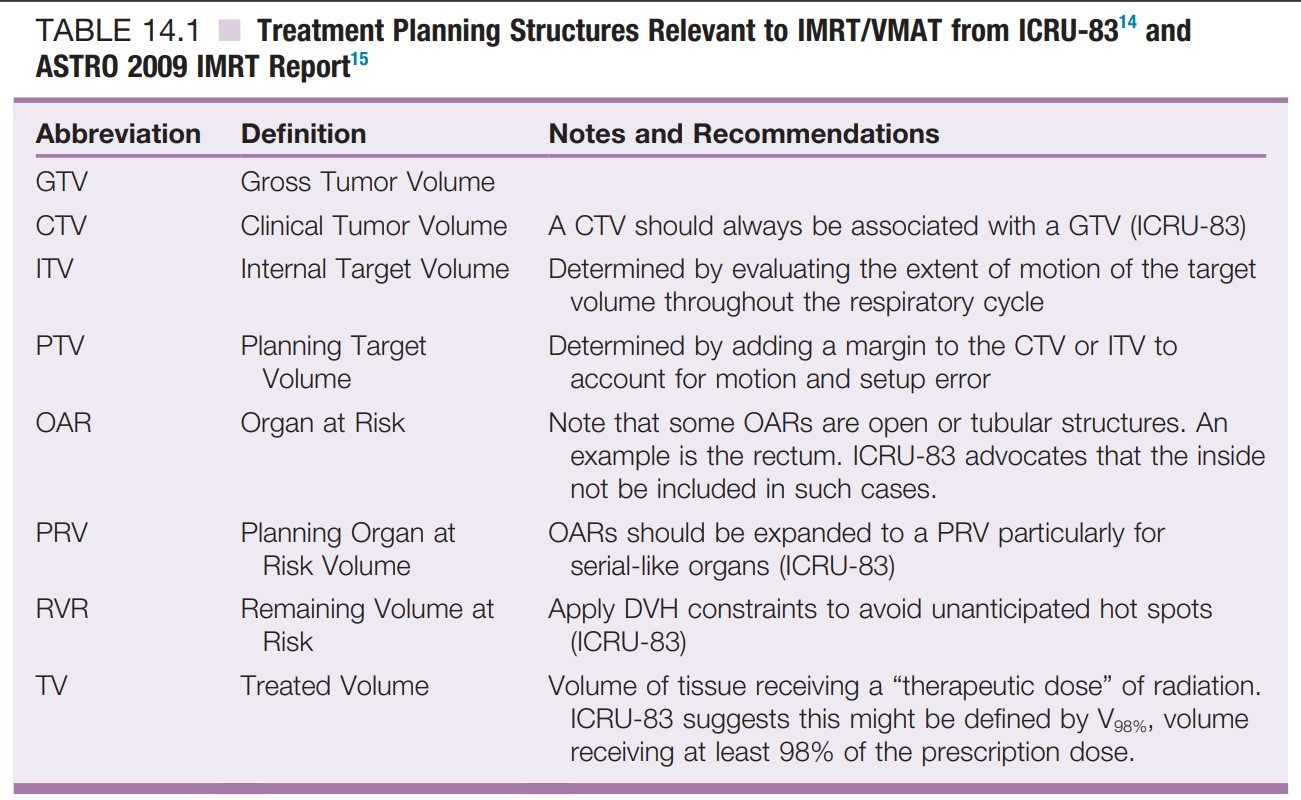
\includegraphics[width=0.8\textwidth]{Imagens/estruturasIcru83.jpg}
		}%
		\caption{Estruturas de planejamento de tratamento relevantes para IMRT/VMAT definidas no ICRU-83.}
		\label{fig:estruturasIcru83}
	\end{figure}

	Em alguns sistemas de planejamento, o processo de delineamento começa com o delineamento do contorno  externo do paciente (body), embora nem todos os sistemas de planejamento exijam essa estrutura. Alguns sistemas fazem o contorno do body automaticamente ao importar a imagem. Nesses casos,  o contorno do body deve ser avaliado para determinar sua precisão, pois essa estrutura determinará a profundidade do tratamento e, finalmente, a MU. As áreas típicas que requerem atenção no contorno do body são as áreas ao redor da boca e do nariz, onde o contorno pode ficar dentro do corpo, ou pode englobar fios ou marcadores colocados na pele além dos dispositivos de imobilização. 

	A maioria dos sistemas de planejamento não leva em consideração qualquer estrutura que estiver fora do contorno corporal (fora do body) e, portanto, os acessórios de imobilização deverão ser contornados e considerados como parte do corpo, caso o impacto dosimétrico desses acessórios deva ser calculado. Alguns sistemas têm a capacidade de adicionar a mesa de tratamento ao conjunto de imagens para contabilizar adequadamente a atenuação no tampo da mesa.

	Alguns sistemas de planejamento (como por exemplo o TomoTherapy e o Pinnacle) consideram cada estrutura dentro do FOV de aquisição e, portanto, calculam inerentemente a atenuação dos dispositivos de imobilização. Um cuidado ao usar um sistema com essa capacidade é que alguns artefatos de imagem da TC criam um anel brilhante ao redor da borda do FOV, que será visto como uma região de alta densidade pelo TPS e a MU será aumentada artificialmente. A avaliação cuidadosa do conjunto de imagens deve ser feita diminuindo o zoom para mostrar o FOV máximo e alternando para uma janela de pulmão para tornar o anel formado mais óbvio. Alguns TPSs têm a capacidade de filtrar artefatos de baixa densidade fora do contorno do corpo aplicando um valor de threshold.

\bibliography{ref.bib}
\end{document}
